\newpage
\section*{ADMINISTRATION API}
%Peter: Give context. Examples!!!
Every software system in a professional environment needs to be maintained by a system administrator.
%Peter: Maintenance free software?
Most applications provide an administrative interface for system administrators to perform these tasks.
\begin{center}
\ding{118} \ding{118} \ding{118}
\end{center}
\textbf{If the administrative interface is a GUI, many of the standard administration tasks can not be easily automated. Repetitive tasks have to be manually completed again and again, which leads to a high frustration of the administrators. It also can be hard to get remote access to such a GUI.}\\

%Peter: Unexpected usage ?? --> Unexpected automation demand
%Peter: System administrators --> Good system administrators
\textit{Unexpected usage.} System administrators have their own ways of organizing their administration tasks. They strive to automate many parts, often in unexpected ways, and a GUI minimizes the possibilities of doing so.\\

\textit{Platform diversity.} The operating systems which administrators are using for their administration tasks often differ from the OS the application to be administered is running on.\\

\textit{Rise of the Cloud} The lower cost to deploy systems in the Cloud leads to more systems being deployed and subsequently to a higher workload for the system administrators if they do not adopt more efficient means for system administration. 
%Rebecca: Did not understand this point: (Christian)
The increase of usage of a resource when technology improves the resources efficiency was shown in 19$^{th}$ century and called "\textit{Jevons Paradox}" \cite{Polimeni2008}. It seems quite likely the same will apply to the number of systems deployed in the Cloud\\

%Peter: The Agile and DevOps --> + Security!!
\textit{Increasing rate of upgrades and deploys} The Agile and DevOps development lifecycles where software upgrades are deployed on a weekly or even a  daily basis, as opposed to the quarterly and yearly deploy cycles of more traditional software development methods, imposes tight control, predictability and efficiency on the deploy, installation and configuration of software. \cite{Humble2010}
\begin{center}
\ding{118} \ding{118} \ding{118} 
\end{center}

\textbf{Therefore: Provide an API for all required administration functionality. Make this API externally available, easily accessible and well documented, so that admins can automate administrative tasks and integrate it easily in the administration processes.}\\

%\textit{Solution in more detail.}

%\textit{Consequences - first positive and then negative, relate these also to the forces}

%The system has to offer the possibility of different administration possibilities, as e.g. a regular %performance check, creation of a new user or a re-start in the case of problems, but also the signalling of a %critical condition. 
%The system has to provide an API (application programming interface) that allows the system administrator to automate system administration tasks. Examples of such tasks are: a regular performance check, creation of a new user or a re-start in the case of problems, but also the signaling of a critical condition.  

Offering an administration API provides much more flexibility for the system administrators to administer the systems in the way they think fits best. It gives them enough freedom to integrate the administration in existing processes. In order to be able to offer this high degree of freedom regarding the usage of the API, the system developers have to carefully design it and to offer the administration functionality in appropriate abstraction levels. This means that the API should be fine-grained enough.
%Unknown1: Contradicts the objectivbe of reuse!! (Abstraction)

%Peter: explain earlier!
The tasks of the system administrators are quite wide e.g.: installation, maintenance, scheduling repair, performance monitoring, backup \& recovery, defining and maintaining usage and security policies etc. For most of these tasks an API can increase the efficiency and quality of the administration processes. 

Automating administrative tasks reduces the number of errors that normally occur in manual execution such as the omission of steps or typing errors in commands. In a script such errors will also occur while programming the script, but once discovered can be fixed for subsequent usage of the script.

Tools for automation can make use of the administration functionality if they can connect to the provided API. For example, the right API helps to automate tasks that are part of a new employee account creation process. \cite{Limoncelli2011a}.

% negative consequences
To securely expose administrative features utilize a {\sc Proxy} \cite{Buschmann1996}. The {\sc Proxy} can include authentication and authorization mechanism and block all unauthorized access attempts, this will be discussed in more detail in the implementation description below.

If the system evolves, the API is also likely to change which might require adaptations the system developers are not aware of. This is a general problem in interface- and component-based development and needs to be addressed in the design of the API too. 

%Peter: or IDE Scram...bin? i.e. Apple interpreter
Providing an API might require more elaborate documentation compared to a more intuitive and self-explaining administrative GUI. For example: an API might require the correct spelling of user roles which need to be assigned to new users. A GUI can offer a selection list including all user roles and possibly an extra explanation of these roles in a separate window section. %Rebecca: what does this mean? (Christian to clarify)
This minimizes the need for extra documentation. The API should therefore include an extensive help, containing all information necessary for using the provided administration functionality. For the same reason the API should include a good exception handling in combination with clear error messages. \\

%\textit{Implementation details, referring back to negative consequences}

In the most simple cases the pattern is a specific variant of a {\sc Service Layer} \cite{Fowler:2002:PEA:579257}. In this case it does not contain any logic, but simply forwards all requests to already existing subsystems that offer the administration functionality. This is shown in Figure \ref{fig:provideAPIDiagram-01}.  

\begin{figure}[h]
\centering
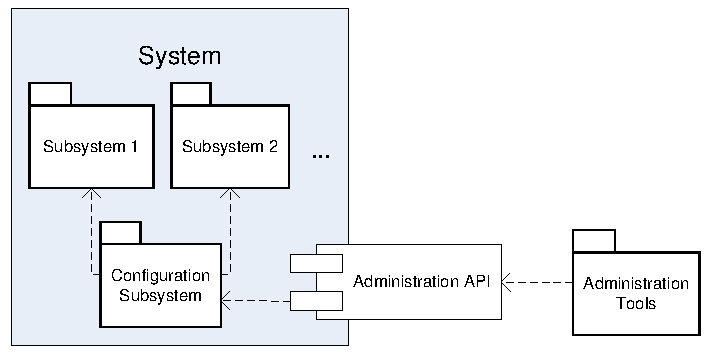
\includegraphics{patterns/provideAPIDiagram-01.pdf}
\caption{Main solution structure of PROVIDE AN ADMINISTRATION API}
\label{fig:provideAPIDiagram-01}
\end{figure}

If the administration API should not be publicly available due to security reasons, a {\sc Proxy} \cite{Buschmann1996} could be used to adequately address this issue. Figure \ref{fig:provideAPIDiagram-02} shows the main design. The protection proxy needs to include some mechanism for authentication and authorization of the requester.

%Peter: ?
These can be implemented making use of e.g. a pattern like {\sc Adapter} \cite{Gamma95} because this pattern can influence the visibility of the administration API with respect to authentication and authorization of the requester.
%(TODO) @Christian: is dit wat je voor ogen hebt?.

%Peter: security patterns! also (w.r.t. Protection Proxy)
\begin{figure}[h]
\centering
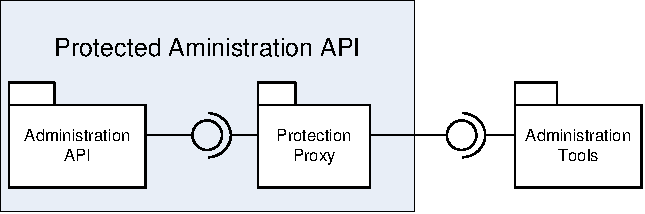
\includegraphics{patterns/provideAPIDiagram-02.pdf}
\caption{An administration API including a protection proxy for security reasons}
\label{fig:provideAPIDiagram-02}
\end{figure}

%Peter: relevant
In certain cases the implementation language of the system and that of the administration API are different. Main reason for this could be that the administration API is required to be provided in a specific scripting language that suits the administrators' tasks best. In that case the administration API subsystem also becomes a specific kind of an {\sc Adapter} \cite{Gamma95} between these two implementation languages.
%Unknown1: missed a three-tiered architecture positioning to style ??

%Peter: separate pattern?
The problem of different platforms used for the system and in the administration environment can be minimized by making use of cross-platform scripting languages like Python, Ruby or TCL. This is also a certain advantage above graphical administration interfaces, as it removes the platform-specific issues caused by the GUI technologies. In combination with such a cross-platform scripting language this pattern shows its real strength as one can uniformly approach the administration API on any given platform.

%Rebecca: I would like to see some concrete example. This is getting pretty abstract: (Christian)
%Peter: Examples - XML, Python(?), JSon. --> Single File Location
Ideally, any changes in the system itself do not lead to changes in the administration API. However, if also functionality of the system regarding its configuration is changing, then also the API likely needs to be changed. The tools of the administrators are dependent on the API both syntactically and semantically in varying degrees. Unfortunately are both dependency types interrelated: the less syntactic the dependency is, the higher it is semantically and vice versa. One criterion that can be used for determining if the API should decrease the syntactic or the semantic dependencies is how easy it is to adapt the connection to the API on either syntactic and semantic level. If the interfaces are easy to adapt on both sides, then one should prefer more syntactically dependent interfaces that explicitly contain the semantic information in the naming of the methods and parameters. If the interfaces are not easy to adapt, then the syntactical dependencies should be low by using more generic interfaces that merely require different parameter contents but no interface adaptations.  

%TODO: some stuff on documentation of the API.


\textit{Microsoft Sharepoint 2013 provides a rich set of APIs. Especially the server object model API offers all required functionality for administration tasks as ``backup, farm health and diagnostics, logging, farm and web application management, upgrade, deployment, caching, and Windows PowerShell customization."\footnote{see \url{http://msdn.microsoft.com/en-us/library/sharepoint/jj164060.aspx}}}

\textit{Another known use of this pattern can be found in Software-Defined Networking. This networking architecture is designed to use standardized APIs for defining and reconfiguring the way data and resources are handled within a network and to make interfacing and reconfiguring the network and its components easier \cite{Kirkpatrick2013}.}

\textit{One possibility of implementing this administrative API in the Java programming language are Java Management Extensions\footnote{\url{http://www.oracle.com/technetwork/java/javase/tech/javamanagement-140525.html}} (JMX). }
%Unknown1: Feedback?? How the patterns improve the architectural design quality regarding the administration point of view?

%
%\begin{center}
%\ding{118} \ding{118} \ding{118} 
%\end{center}
%
%\textit{Rationale?}\\
%%Using this pattern will make the life of a system administrator more pleasant, especially in cross-platform situations, as it removes the platform-specific issues caused by a graphical administration interface. In combination with a cross-platform scripting language (e.g. Python, Ruby, TCL) this pattern shows its real strength as one can uniformly approach the administration API on any given platform.
%
